\section{Analysis of covariance}
\frame{\sectionpage}



\begin{frame}[fragile]{Analysis of covariance}

  \begin{itemize}
  \item ANOVA: explanatory variables categorical (divide data into groups)
  \item traditionally, analysis of covariance has categorical $x$'s plus one numerical $x$ (``covariate'') to be adjusted for.
  \item \texttt{lm} handles this too.
  \item Simple example: two treatments (drugs) (\verb-a- and \verb-b-), with before and after scores. 
    \begin{itemize}
    \item 
Does knowing before score and/or treatment help to predict after score?
\item Is after score different by treatment/before score?
    \end{itemize}
  \end{itemize}

\end{frame}

\begin{frame}[fragile]{Data}

Treatment, before, after:

\begin{multicols}{2}

\begin{verbatim}
a 5 20
a 10 23
a 12 30
a 9 25
a 23 34
a 21 40
a 14 27
a 18 38
a 6 24
a 13 31
b 7 19
b 12 26
b 27 33
b 24 35
b 18 30
b 22 31
b 26 34
b 21 28
b 14 23
b 9 22
\end{verbatim}

  
\end{multicols}

\end{frame}


\begin{frame}[fragile]{Making a plot}

  \begin{footnotesize}

    
  \end{footnotesize}
 
\begin{knitrout}
\definecolor{shadecolor}{rgb}{0.969, 0.969, 0.969}\color{fgcolor}\begin{kframe}
\begin{alltt}
\hlstd{prepost}\hlkwb{=}\hlkwd{read.table}\hlstd{(}\hlstr{"ancova.txt"}\hlstd{,}\hlkwc{header}\hlstd{=T)}
\hlkwd{str}\hlstd{(prepost)}
\end{alltt}
\begin{verbatim}
## 'data.frame':	20 obs. of  3 variables:
##  $ drug  : Factor w/ 2 levels "a","b": 1 1 1 1 1 1 1 1 1 1 ...
##  $ before: int  5 10 12 9 23 21 14 18 6 13 ...
##  $ after : int  20 23 30 25 34 40 27 38 24 31 ...
\end{verbatim}
\end{kframe}
\end{knitrout}
  
\begin{knitrout}
\definecolor{shadecolor}{rgb}{0.969, 0.969, 0.969}\color{fgcolor}\begin{kframe}
\begin{alltt}
\hlstd{g}\hlkwb{=}\hlkwd{ggplot}\hlstd{(prepost,}\hlkwd{aes}\hlstd{(}\hlkwc{x}\hlstd{=before,}\hlkwc{y}\hlstd{=after,}\hlkwc{colour}\hlstd{=drug))}\hlopt{+}
  \hlkwd{geom_point}\hlstd{()}
\end{alltt}
\end{kframe}
\end{knitrout}
  
  
\end{frame}

\begin{frame}{The plot}

 
\begin{knitrout}
\definecolor{shadecolor}{rgb}{0.969, 0.969, 0.969}\color{fgcolor}\begin{kframe}
\begin{alltt}
\hlstd{g}
\end{alltt}
\end{kframe}
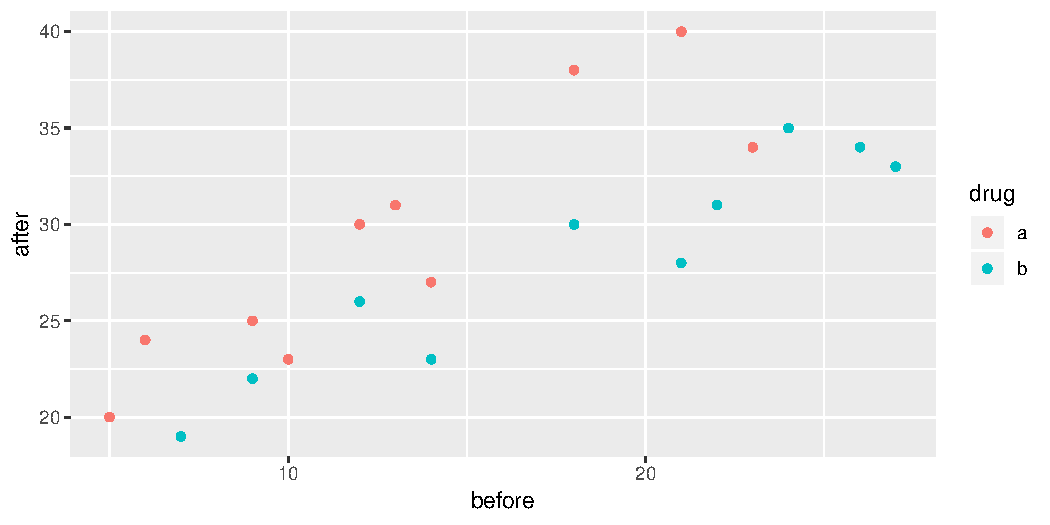
\includegraphics[width=\maxwidth]{figure/spizzo-1} 

\end{knitrout}
  
  
\end{frame}

\begin{frame}[fragile]{Comments}

\begin{knitrout}
\definecolor{shadecolor}{rgb}{0.969, 0.969, 0.969}\color{fgcolor}\begin{kframe}
\begin{alltt}
\hlstd{g}
\end{alltt}
\end{kframe}
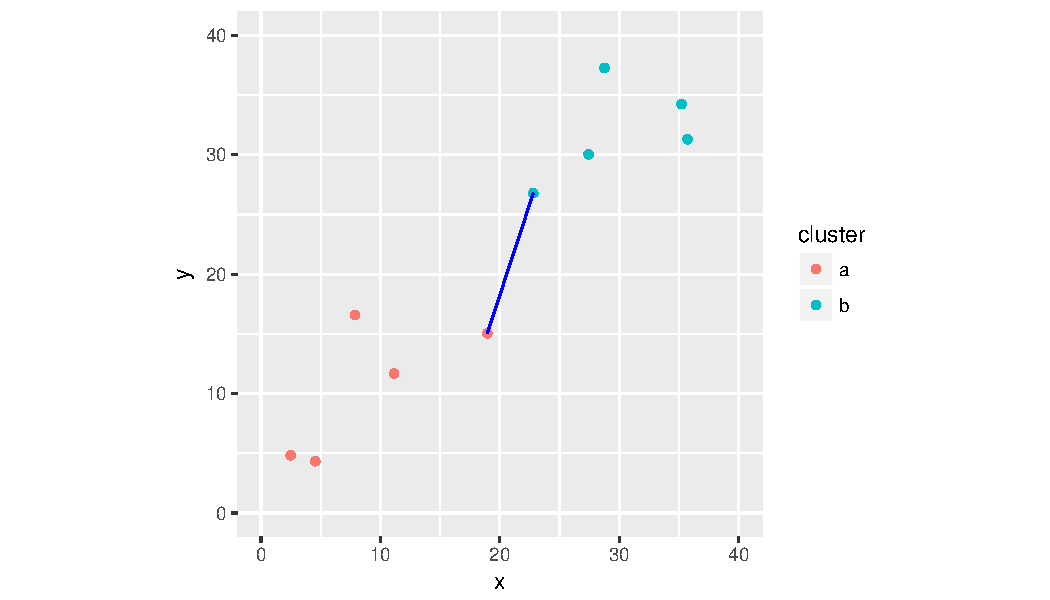
\includegraphics[width=\maxwidth]{figure/unnamed-chunk-3-1} 

\end{knitrout}

\begin{itemize}
\item As before score goes up, after score goes up.
\item Red points (drug A) generally above blue points (drug B), for
  comparable before score.
\item Suggests before score effect \emph{and} drug effect.
\end{itemize}
  
\end{frame}


\begin{frame}[fragile]{The means}

 
\begin{knitrout}
\definecolor{shadecolor}{rgb}{0.969, 0.969, 0.969}\color{fgcolor}\begin{kframe}
\begin{alltt}
\hlstd{prepost} \hlopt \hlkwd{group_by}\hlstd{(drug)} \hlopt
  \hlkwd{summarize}\hlstd{(}\hlkwc{before_mean}\hlstd{=}\hlkwd{mean}\hlstd{(before),}
            \hlkwc{after_mean}\hlstd{=}\hlkwd{mean}\hlstd{(after)}
           \hlstd{)}
\end{alltt}
\begin{verbatim}
## # A tibble: 2 × 3
##     drug before_mean after_mean
##   <fctr>       <dbl>      <dbl>
## 1      a        13.1       29.2
## 2      b        18.0       28.1
\end{verbatim}
\end{kframe}
\end{knitrout}
  

\begin{itemize}
\item Mean ``after'' score slightly higher for treatment A.
\item Mean ``before'' score much higher for treatment B.
\item Greater {\em improvement} on treatment A. 
\end{itemize}
  
\end{frame}

\begin{frame}[fragile]{Testing for interaction}

 
\begin{knitrout}
\definecolor{shadecolor}{rgb}{0.969, 0.969, 0.969}\color{fgcolor}\begin{kframe}
\begin{alltt}
\hlstd{prepost.1}\hlkwb{=}\hlkwd{lm}\hlstd{(after}\hlopt{~}\hlstd{before}\hlopt{*}\hlstd{drug,}\hlkwc{data}\hlstd{=prepost)}
\hlkwd{anova}\hlstd{(prepost.1)}
\end{alltt}
\begin{verbatim}
## Analysis of Variance Table
## 
## Response: after
##             Df Sum Sq Mean Sq F value    Pr(>F)    
## before       1 430.92  430.92 62.6894  6.34e-07 ***
## drug         1 115.31  115.31 16.7743 0.0008442 ***
## before:drug  1  12.34   12.34  1.7948 0.1990662    
## Residuals   16 109.98    6.87                      
## ---
## Signif. codes:  0 '***' 0.001 '**' 0.01 '*' 0.05 '.' 0.1 ' ' 1
\end{verbatim}
\end{kframe}
\end{knitrout}


\begin{itemize}
\item Interaction not significant. Will remove later.
\end{itemize}
\end{frame}



\begin{frame}[fragile]{Predictions, with interaction included}


  
  \begin{multicols}{2}
    

  
  Make combinations of before score and drug:
  
\begin{knitrout}
\definecolor{shadecolor}{rgb}{0.969, 0.969, 0.969}\color{fgcolor}\begin{kframe}
\begin{alltt}
\hlstd{new}\hlkwb{=}\hlkwd{expand.grid}\hlstd{(}
      \hlkwc{before}\hlstd{=}\hlkwd{c}\hlstd{(}\hlnum{5}\hlstd{,}\hlnum{15}\hlstd{,}\hlnum{25}\hlstd{),}
      \hlkwc{drug}\hlstd{=}\hlkwd{c}\hlstd{(}\hlstr{"a"}\hlstd{,}\hlstr{"b"}\hlstd{)}
               \hlstd{)}
\hlstd{new}
\end{alltt}
\begin{verbatim}
##   before drug
## 1      5    a
## 2     15    a
## 3     25    a
## 4      5    b
## 5     15    b
## 6     25    b
\end{verbatim}
\end{kframe}
\end{knitrout}

Do predictions:

\begin{knitrout}
\definecolor{shadecolor}{rgb}{0.969, 0.969, 0.969}\color{fgcolor}\begin{kframe}
\begin{alltt}
\hlstd{pred}\hlkwb{=}\hlkwd{predict}\hlstd{(prepost.1,new)}
\hlstd{preds}\hlkwb{=}\hlkwd{data.frame}\hlstd{(new,pred)}
\hlstd{preds}
\end{alltt}
\begin{verbatim}
##   before drug     pred
## 1      5    a 21.29948
## 2     15    a 31.05321
## 3     25    a 40.80693
## 4      5    b 18.71739
## 5     15    b 25.93478
## 6     25    b 33.15217
\end{verbatim}
\end{kframe}
\end{knitrout}
  
  \end{multicols}

\end{frame}

\begin{frame}[fragile]{Making a plot with lines for each \texttt{drug}}

 
\begin{knitrout}
\definecolor{shadecolor}{rgb}{0.969, 0.969, 0.969}\color{fgcolor}\begin{kframe}
\begin{alltt}
\hlstd{g}\hlkwb{=}\hlkwd{ggplot}\hlstd{(prepost,}
  \hlkwd{aes}\hlstd{(}\hlkwc{x}\hlstd{=before,}\hlkwc{y}\hlstd{=after,}\hlkwc{colour}\hlstd{=drug))}\hlopt{+}
  \hlkwd{geom_point}\hlstd{()}\hlopt{+}
  \hlkwd{geom_line}\hlstd{(}\hlkwc{data}\hlstd{=preds,}\hlkwd{aes}\hlstd{(}\hlkwc{y}\hlstd{=pred))}
\end{alltt}
\end{kframe}
\end{knitrout}


\begin{itemize}
\item Last line could (more easily) be 

\begin{knitrout}
\definecolor{shadecolor}{rgb}{0.969, 0.969, 0.969}\color{fgcolor}\begin{kframe}
\begin{alltt}
\hlkwd{geom_smooth}\hlstd{(}\hlkwc{method}\hlstd{=}\hlstr{"lm"}\hlstd{,}\hlkwc{se}\hlstd{=F)}
\end{alltt}
\end{kframe}
\end{knitrout}

which would work here, but not for later plot.
\item Here, final line:
  \begin{itemize}
  \item   joins points by lines \emph{for different data
    set} (\texttt{preds} rather than \texttt{prepost}),
\item   \emph{different $y$} (\texttt{pred} rather than \texttt{after}),
  
\item but same $x$ (\texttt{x=before} inherited from first \texttt{aes}).

  \end{itemize}
  
\end{itemize}
  
  
\end{frame}

\begin{frame}[fragile]{The plot}
 
  
\begin{knitrout}
\definecolor{shadecolor}{rgb}{0.969, 0.969, 0.969}\color{fgcolor}\begin{kframe}
\begin{alltt}
\hlstd{g}
\end{alltt}
\end{kframe}
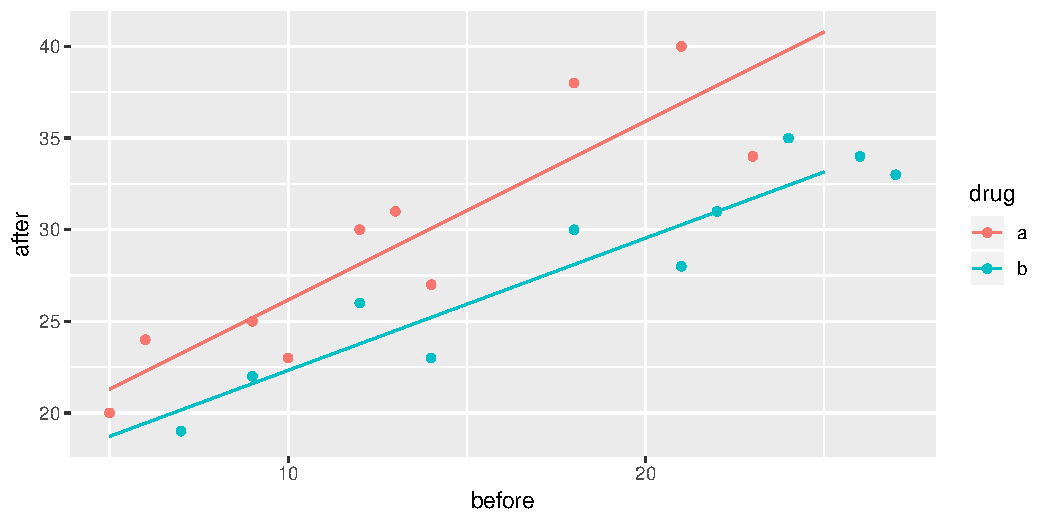
\includegraphics[width=\maxwidth]{figure/nachwazzo-1} 

\end{knitrout}
   
   
 
 \begin{itemize}
 \item Lines almost parallel, but not quite.
 \item Non-parallelism (interaction) not significant.
 \end{itemize}
   
\end{frame}
 

\begin{frame}[fragile]{Taking out interaction}


{\small
  
 
\begin{knitrout}
\definecolor{shadecolor}{rgb}{0.969, 0.969, 0.969}\color{fgcolor}\begin{kframe}
\begin{alltt}
\hlstd{prepost.2}\hlkwb{=}\hlkwd{lm}\hlstd{(after}\hlopt{~}\hlstd{before}\hlopt{+}\hlstd{drug,}\hlkwc{data}\hlstd{=prepost)}
\hlkwd{anova}\hlstd{(prepost.2)}
\end{alltt}
\begin{verbatim}
## Analysis of Variance Table
## 
## Response: after
##           Df Sum Sq Mean Sq F value    Pr(>F)    
## before     1 430.92  430.92  59.890 5.718e-07 ***
## drug       1 115.31  115.31  16.025 0.0009209 ***
## Residuals 17 122.32    7.20                      
## ---
## Signif. codes:  0 '***' 0.001 '**' 0.01 '*' 0.05 '.' 0.1 ' ' 1
\end{verbatim}
\end{kframe}
\end{knitrout}
}
  
  \begin{itemize}
  \item Take out non-significant interaction.
  \item \texttt{before} and \texttt{drug} strongly significant.
  \item Do predictions again and plot them.
  \end{itemize}
  
\end{frame}

\begin{frame}[fragile]{Predicted values again (no-interaction model)}

   
\begin{knitrout}
\definecolor{shadecolor}{rgb}{0.969, 0.969, 0.969}\color{fgcolor}\begin{kframe}
\begin{alltt}
\hlstd{pred}\hlkwb{=}\hlkwd{predict}\hlstd{(prepost.2,new)}
\hlstd{preds}\hlkwb{=}\hlkwd{data.frame}\hlstd{(new,pred)}
\hlstd{preds}
\end{alltt}
\begin{verbatim}
##   before drug     pred
## 1      5    a 22.49740
## 2     15    a 30.77221
## 3     25    a 39.04703
## 4      5    b 17.34274
## 5     15    b 25.61756
## 6     25    b 33.89237
\end{verbatim}
\end{kframe}
\end{knitrout}
 

Each increase of 10 in before score results in 8.3 in predicted after
score, \emph{the same for both drugs}.
  
\end{frame}

\begin{frame}[fragile]{Making a plot, again}

 
\begin{knitrout}
\definecolor{shadecolor}{rgb}{0.969, 0.969, 0.969}\color{fgcolor}\begin{kframe}
\begin{alltt}
\hlstd{g}\hlkwb{=}\hlkwd{ggplot}\hlstd{(prepost,}
  \hlkwd{aes}\hlstd{(}\hlkwc{x}\hlstd{=before,}\hlkwc{y}\hlstd{=after,}\hlkwc{colour}\hlstd{=drug))}\hlopt{+}
  \hlkwd{geom_point}\hlstd{()}\hlopt{+}
  \hlkwd{geom_line}\hlstd{(}\hlkwc{data}\hlstd{=preds,}\hlkwd{aes}\hlstd{(}\hlkwc{y}\hlstd{=pred))}
\end{alltt}
\end{kframe}
\end{knitrout}
 

Exactly same as before, but using new predictions.
  
\end{frame}

\begin{frame}{The no-interaction plot of predicted values}
  
 
\begin{knitrout}
\definecolor{shadecolor}{rgb}{0.969, 0.969, 0.969}\color{fgcolor}\begin{kframe}
\begin{alltt}
\hlstd{g}
\end{alltt}
\end{kframe}
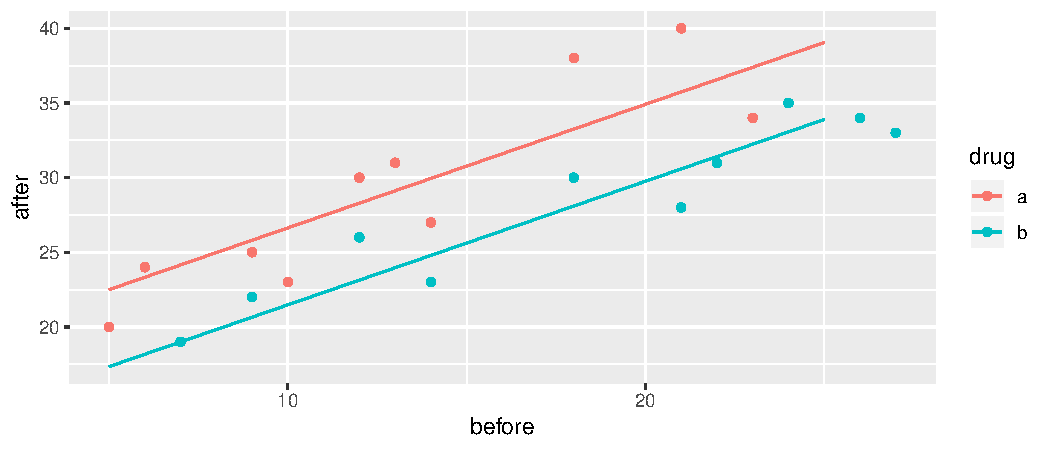
\includegraphics[width=\maxwidth]{figure/cabazzo-1} 

\end{knitrout}


Note that lines now \emph{parallel}. No-interaction model forces them
to have the same slope. 

\end{frame}

\begin{frame}[fragile]{Different look at model output}
  
  \begin{itemize}
  \item \texttt{anova(prepost.2)} tests for significant effect of
    before score and of drug, but doesn't help with interpretation.
  \item \texttt{summary(prepost.2)} views as regression with slopes:
    
    \begin{scriptsize}
\begin{knitrout}
\definecolor{shadecolor}{rgb}{0.969, 0.969, 0.969}\color{fgcolor}\begin{kframe}
\begin{alltt}
\hlkwd{summary}\hlstd{(prepost.2)}
\end{alltt}
\begin{verbatim}
## 
## Call:
## lm(formula = after ~ before + drug, data = prepost)
## 
## Residuals:
##     Min      1Q  Median      3Q     Max 
## -3.6348 -2.5099 -0.2038  1.8871  4.7453 
## 
## Coefficients:
##             Estimate Std. Error t value Pr(>|t|)    
## (Intercept)  18.3600     1.5115  12.147 8.35e-10 ***
## before        0.8275     0.0955   8.665 1.21e-07 ***
## drugb        -5.1547     1.2876  -4.003 0.000921 ***
## ---
## Signif. codes:  0 '***' 0.001 '**' 0.01 '*' 0.05 '.' 0.1 ' ' 1
## 
## Residual standard error: 2.682 on 17 degrees of freedom
## Multiple R-squared:  0.817,	Adjusted R-squared:  0.7955 
## F-statistic: 37.96 on 2 and 17 DF,  p-value: 5.372e-07
\end{verbatim}
\end{kframe}
\end{knitrout}
    \end{scriptsize}
  \end{itemize}
  
\end{frame}

\begin{frame}[fragile]{Understanding those slopes}
  
  \begin{scriptsize}
\begin{knitrout}
\definecolor{shadecolor}{rgb}{0.969, 0.969, 0.969}\color{fgcolor}\begin{kframe}
\begin{alltt}
\hlkwd{summary}\hlstd{(prepost.2)}\hlopt{$}\hlstd{coefficients}
\end{alltt}
\begin{verbatim}
##               Estimate Std. Error   t value     Pr(>|t|)
## (Intercept) 18.3599949 1.51153263 12.146608 8.354496e-10
## before       0.8274813 0.09550226  8.664520 1.211339e-07
## drugb       -5.1546584 1.28765245 -4.003144 9.209111e-04
\end{verbatim}
\end{kframe}
\end{knitrout}
%$ %$ %$
  \end{scriptsize}

\begin{itemize}
\item \texttt{before} ordinary numerical variable; \texttt{drug}
  categorical. 
\item \texttt{lm} uses first category \texttt{druga} as baseline.
\item Intercept is prediction of after score for before score 0 and
  \emph{drug A}.
\item \texttt{before} slope is predicted change in after score when
  before score increases by 1 (usual slope)
\item Slope for \texttt{drugb} is \emph{change} in predicted after
  score for being on drug B rather than drug A. Same for \emph{any}
  before score (no interaction).
\item In \texttt{summary(prepost.1)}, \texttt{before:drugb} would be change in
  \emph{slope} for being on drug B rather than A.
  
\end{itemize}

  
\end{frame}

\begin{frame}[fragile]{Summary}

  \begin{itemize}
  \item ANCOVA model: fits different regression line for each group,
    predicting response from covariate.
  \item ANCOVA model with interaction between factor and covariate
    allows different slopes for each line.
  \item Sometimes those lines can cross over!
  \item If interaction not significant, take out. Lines then parallel.
  \item With parallel lines, groups have consistent effect regardless
    of value of covariate.
  \end{itemize}
  
\end{frame}
